%% chapter3_slides.tex
%% Chapter 3: The Krasnosel'ski\u{i}-Mann Iteration
%% Dong, Cho, He, Pardalos & Rassias --- The Krasnosel'ski\u{i}-Mann Iterative Method (SpringerBriefs in Optimization, 2022)
%% Compile: pdflatex -interaction=nonstopmode chapter3_slides.tex  (run twice)

\documentclass[aspectratio=169,10pt]{beamer}

\usetheme{Madrid}
\usecolortheme{seahorse}
\usefonttheme{professionalfonts}
\setbeamertemplate{footline}[frame number]
\setbeamertemplate{navigation symbols}{}

%% Packages
\usepackage{amsmath,amssymb,mathtools}
\usepackage{graphicx}
\usepackage{listings}
\usepackage{xcolor}
\usepackage{booktabs}
\usepackage{microtype}

\graphicspath{{figures/}}

%% Python listings style
\lstdefinestyle{python}{
  language=Python,
  basicstyle=\ttfamily\scriptsize,
  keywordstyle=\color{blue!80!black}\bfseries,
  commentstyle=\color{green!50!black}\itshape,
  stringstyle=\color{orange!80!black},
  numbers=left,
  numberstyle=\tiny\color{gray},
  stepnumber=1,
  numbersep=4pt,
  frame=single,
  backgroundcolor=\color{gray!7},
  breaklines=true,
  showstringspaces=false,
  tabsize=4,
  captionpos=b,
}

%% Maths shortcuts
\newcommand{\cH}{\mathcal{H}}
\newcommand{\Fix}{\operatorname{Fix}}
\newcommand{\R}{\mathbb{R}}
\newcommand{\N}{\mathbb{N}}
\newcommand{\norm}[1]{\left\|#1\right\|}
\newcommand{\inner}[2]{\left\langle #1, #2 \right\rangle}
\newcommand{\weakto}{\rightharpoonup}

%% Title info
\title[KM Method -- Ch.3]{The Krasnosel'ski\u{i}-Mann Iterative Method}
\subtitle{Chapter 3: The Krasnosel'ski\u{i}-Mann Iteration}
\author{Based on Dong, Cho, He, Pardalos \& Rassias}
\institute{SpringerBriefs in Optimization, 2022}
\date{}

% ---------------------------------------------------------------
\begin{document}
% ---------------------------------------------------------------

\begin{frame}
  \titlepage
\end{frame}

\begin{frame}{Chapter Outline}
  \tableofcontents
\end{frame}

% =================================================================
\section{Recap and New Notation}
% =================================================================

\begin{frame}[allowframebreaks]{Notation You'll Need / Recap}

  \textbf{From Chapter 2 (recap).} Let $\cH$ be a real Hilbert space
  with inner product $\inner{\cdot}{\cdot}$ and norm $\norm{\cdot}$.
  For $T:\cH\to\cH$ (or $T:C\to C$ on a closed convex subset $C$):
  \begin{itemize}
    \item $T$ is \textbf{nonexpansive} if $\norm{T(x)-T(y)}\le\norm{x-y}$
      for all $x,y$.
    \item $\Fix(T)=\{x : T(x)=x\}$ is the set of \textbf{fixed points}.
    \item $\{x_n\}$ \textbf{converges weakly} to $x^*$ (written
      $x_n \weakto x^*$) if $\inner{x_n}{z}\to \inner{x^*}{z}$ for every
      $z\in\cH$; it converges \textbf{strongly} (in norm) if
      $\norm{x_n-x^*}\to 0$. Strong convergence always implies weak
      convergence, not conversely (in infinite dimensions).
    \item The \textbf{Picard iteration} is the naive scheme
      $x_{n+1}=T(x_n)$; it need not converge even when $T$ is
      nonexpansive and has a fixed point (e.g.\ a rotation).
  \end{itemize}

  \framebreak

  \textbf{New in this chapter.}
  \begin{itemize}
    \item The \textbf{relaxation (or averaging) sequence} $\{\lambda_n\}\subset[0,1]$
      blends the current point $x_n$ with the Picard step $T(x_n)$:
      $$x_{n+1}=(1-\lambda_n)x_n+\lambda_n T(x_n).$$
      $\lambda_n=1$ recovers pure Picard; $\lambda_n=0$ means ``don't move.''
    \item The \textbf{perturbation term} $e_n$ (or the pair $e_n^1,e_n^2$)
      models computational error in evaluating $x_n$ or $T(x_n)$ at each
      step; it is required to be \textbf{summable},
      $\sum_{n}\norm{e_n}<+\infty$, so that the accumulated error over
      infinitely many steps stays finite.
    \item \textbf{Convergence rate $O(1/\sqrt n)$ (plain terms):} the
      residual that measures how far $x_n$ is from being a fixed point
      (e.g.\ $\norm{x_n-T(x_n)}$) shrinks no slower than a constant times
      $1/\sqrt n$. Doubling the iteration budget only shrinks the
      guaranteed error bound by a factor $1/\sqrt2\approx0.71$ --- far
      slower than the geometric (linear) rates you may know from
      contraction mappings, where doubling the budget can shrink the
      error by many orders of magnitude. This \emph{sublinear} rate is
      the price paid for working with mere nonexpansive maps instead of
      contractions.
  \end{itemize}

  \framebreak

  \textbf{Running example (used throughout this chapter).}
  Let $\cH=\R^2$, $C=$ closed unit disk, and
  $$T(x)=\begin{cases}x/\norm{x}, & \norm{x}>1,\\ x, & \norm{x}\le 1,\end{cases}$$
  the metric projection onto $C$ (firmly nonexpansive, hence nonexpansive,
  $\Fix(T)=C$). Start at $x_0=(3,4)$, $\norm{x_0}=5$. Every iterate stays
  on the ray through $x_0$, so the \emph{unique} point of $\Fix(T)$ that
  the KM sequence can reach along that ray is
  $$x^*=x_0/\norm{x_0}=(0.6,0.8).$$
  Writing $x_n=r_n\,(0.6,0.8)$, the vector recursion collapses to the
  scalar recursion (derived in Chapter 1)
  $$r_{n+1}=(1-\lambda_n)r_n+\lambda_n, \qquad r_0=5.$$
  We will plug in constant and decreasing $\{\lambda_n\}$ throughout.
\end{frame}

% =================================================================
\section{3.1 The Original Krasnosel'ski\u{i}-Mann Iteration}
% =================================================================

\begin{frame}[allowframebreaks]{3.1 The KM Iteration: Definition}

  \begin{block}{Krasnosel'ski\u{i}-Mann (KM) iteration (3.1)}
    Let $X$ be a normed space, $C\subset X$ convex, $T:C\to C$ an
    operator, and $\{\lambda_n\}\subset[0,1]$ a real sequence. Starting
    from any $x_0\in C$,
    $$x_{n+1}=(1-\lambda_n)x_n+\lambda_n T(x_n) \quad\text{for each } n\ge0.$$
    \emph{Symbols:} $x_n$ = current iterate; $T(x_n)$ = one Picard step
    from $x_n$; $\lambda_n$ = how much of the Picard step to take (the
    \emph{relaxation parameter}).
  \end{block}

  \textbf{Intuition.} At each step you take a weighted average
  (a ``relaxed'' step) between staying put and moving all the way to
  $T(x_n)$. Mann introduced this in 1953; Krasnosel'ski\u{i} (1955)
  studied the special case of \emph{constant} $\lambda_n\equiv\lambda$.
  Some authors call it the Mann--Toeplitz process, since Toeplitz
  studied a more general matrix approach of which (3.1) is a special
  case.

  \framebreak

  \textbf{Why not just use Picard ($\lambda_n\equiv1$)?} Nonexpansive
  maps can have rotation-like behaviour with no attraction toward the
  fixed point, so $x_{n+1}=T(x_n)$ can cycle forever without converging.
  Averaging with the identity (any $\lambda_n<1$) damps that
  oscillation --- this is the entire point of the KM scheme.

  \textbf{Running example, constant $\lambda=0.5$.} Using
  $r_{n+1}=(1-\lambda)r_n+\lambda$ with $r_0=5$:
  $$r_0=5,\ r_1=3,\ r_2=2,\ r_3=1.5,\ r_4=1.25,\ r_5=1.125,\ \dots \to 1.$$
  In fact $e_n:=r_n-1$ satisfies $e_{n+1}=(1-\lambda)e_n$, so
  $e_n=4\cdot0.5^n$: \textbf{geometric} (linear) decay to the fixed
  point $x^*=(0.6,0.8)$.
\end{frame}

\begin{frame}[allowframebreaks]{3.1 Mann's Original Matrix Formulation}

  Mann's 1953 paper phrased the iteration through an infinite
  lower-triangular matrix $A=(a_{nk})$ satisfying
  \begin{itemize}
    \item (A1) $a_{nk}\ge0$ for $n,k\ge1$ and $a_{nk}=0$ for $k>n$;
    \item (A2) $\sum_{k=1}^n a_{nk}=1$ for each $n\ge1$ (each row is a
      convex-combination weight vector).
  \end{itemize}

  \begin{block}{Generalized Mann process (3.2)}
    Starting from $x_1\in C$,
    $$v_n=\sum_{k=1}^{n}a_{nk}x_k, \qquad x_{n+1}=T(v_n).$$
  \end{block}
  Here $v_n$ is a weighted \emph{centroid} of all past iterates
  $x_1,\dots,x_n$, and the $(n{+}1)$-st iterate is the image of that
  centroid under $T$. This is denoted briefly $(x_1,A,T)$; when $A=I$
  (identity) it reduces to plain Picard iteration.

  \begin{block}{Theorem 3.1 (Mann)}
    Let $C$ be convex compact in a Banach space, $T:C\to C$
    nonexpansive. If either $\{x_n\}$ or $\{v_n\}$ converges, then the
    other also converges, to the \emph{same} limit, and that limit is a
    fixed point of $T$.
  \end{block}

  \framebreak

  \begin{block}{The Ces\`aro matrix $\Lambda$ (a particular $A$)}
    $\Lambda_{nk}=\dfrac1n$ for $1\le k\le n$. Process (3.3):
    $$v_n=\frac1n\sum_{k=1}^n x_k, \qquad x_{n+1}=T(v_n).$$
    One checks algebraically that this is equivalent to the
    \emph{relaxed} recursion (3.4)
    $$v_{n+1}=\Bigl(1-\frac{1}{n+1}\Bigr)v_n+\frac{1}{n+1}T(v_n),$$
    i.e.\ exactly a KM iteration (3.1) with the \emph{decreasing}
    relaxation sequence $\lambda_n=\tfrac{1}{n+1}$.
  \end{block}

  \textbf{Running example, decreasing $\lambda_n=\frac{1}{n+2}$.}
  (Shifting the index by one to avoid the boundary case $\lambda=1$ at
  the very first step.) Using $r_{n+1}=(1-\lambda_n)r_n+\lambda_n$:
  $$r_0=5,\ r_1=3,\ r_2=2.333,\ r_3=2,\ r_4=1.8,\ r_5=1.667,\dots$$
  One can check directly $e_n=r_n-1=\dfrac{4}{n+1}$ \textbf{exactly} ---
  only \textbf{sublinear} ($O(1/n)$) decay: much slower than the
  geometric decay of constant $\lambda=0.5$, even though both converge.
\end{frame}

\begin{frame}[allowframebreaks]{3.1 Convergence for Continuous Scalar $T$}

  \begin{block}{Theorem 3.2 (Mann, \emph{[141, Thm.\ 4]})}
    If $T:[a,b]\to[a,b]$ is continuous with a \emph{unique} fixed
    point $p$, then $\{x_n\}$ from the Ces\`aro process (3.3) converges
    to $p$ for every starting point $x_1\in[a,b]$.
  \end{block}

  Franks and Marzec later removed the uniqueness assumption. Borwein
  and Borwein generalized further: let $\{d_n\}$ be nonnegative with
  $d_1>0$, $\sum_{k=1}^{+\infty}d_k=+\infty$, and set
  $a_{nk}=d_k/\sum_{k=1}^n d_k$.

  \begin{block}{Theorem 3.3 (\emph{[20, Thm.\ 11]})}
    If $T:[a,b]\to[a,b]$ has $\Fix(T)\ne\emptyset$, then $\{x_n\}$ from
    (3.2) converges to a fixed point of $T$ provided \textbf{either}
    \begin{enumerate}
      \item[(a)] $T$ is continuous and $\displaystyle\lim_{n\to\infty}a_{nn}=0$; \textbf{or}
      \item[(b)] $T$ is $L$-Lipschitz and
        $\displaystyle\limsup_{n\to\infty}a_{nn}\le\frac{2}{L+1}$.
    \end{enumerate}
  \end{block}
  The Ces\`aro matrix satisfies (a). \emph{Warning:} Theorem 3.3 fails
  in higher-dimensional spaces (a counterexample exists).

  \framebreak

  \textbf{Dotson's ``normal Mann process.''} Add to (A1)--(A2):
  \begin{itemize}
    \item (A3) $\lim_{n\to\infty}a_{nk}=0$ for each fixed $k$;
    \item (A4) $a_{n+1,k}=(1-a_{n+1,n+1})a_{nk}$ for $1\le k\le n$.
  \end{itemize}
  Condition (A4) lets you unwind $v_{n+1}$ as a genuine two-term
  relaxation:
  $$v_{n+1}=a_{n+1,n+1}Tv_n+(1-a_{n+1,n+1})v_n
           =\lambda_n T(v_n)+(1-\lambda_n)v_n,$$
  where $\lambda_n:=a_{n+1,n+1}$ is read off the \emph{main diagonal} of
  $A$. So \emph{every} normal Mann process is secretly a KM iteration
  (3.1) with this particular diagonal relaxation sequence. This is why
  it is sometimes called the ``Mann--Dotson'' iterate, even though it is
  a special case of (3.2).
\end{frame}

\begin{frame}[allowframebreaks]{3.1 Relaxed Mean Iteration and Concentrating Arrays}

  Combettes and Pennanen generalized (3.2) to an \emph{inexact}, relaxed
  version for a finite family of operators; the single-operator exact
  case is:

  \begin{block}{Relaxed mean iteration scheme (3.5)}
    $$v_n=\sum_{k=0}^{n}a_{nk}x_k, \qquad
      x_{n+1}=(1-\lambda_n)v_n+\lambda_n T(v_n).$$
    Reduces to the mean iteration (3.2) when $\lambda_n\equiv1$.
  \end{block}

  \begin{block}{Definition 3.1 (Concentrating array, condition (A5))}
    The array $\{a_{nk}\}$ is \emph{concentrating} if every nonnegative
    sequence $\{\xi_n\}$ satisfying
    $$\xi_{n+1}\le\sum_{k=0}^n a_{nk}\xi_k \quad\text{for each } n\ge0$$
    converges. \emph{Intuition:} if a nonnegative quantity is bounded
    above by a weighted average of its own past values under this
    array, that quantity is forced to settle down --- exactly the kind
    of ``monotone-ish'' control we will exploit for $\norm{x_n-p}$.
  \end{block}

  \framebreak

  \begin{block}{Theorem 3.4 (\emph{[46, Thm.\ 3.5]})}
    Let $\{\lambda_n\}\subset[\delta,2-\delta]$ for some $\delta\in(0,2)$.
    Suppose $\{a_{nk}\}$ satisfies (A1)--(A3) and (A5), and
    $T:\cH\to\cH$ is \textbf{firmly nonexpansive} with $\Fix(T)\ne\emptyset$.
    Then $\{x_n\}$ from (3.5) \textbf{weakly converges} to a fixed
    point of $T$.
  \end{block}

  Combettes and Glaudin later dropped condition (A1) (nonnegativity),
  moving from a \emph{convex}-hull iteration to an \emph{affine}-hull
  iteration, under assumptions (B1)--(B4) (boundedness of row sums of
  absolute values, row sums $=1$, columns $\to0$, and a concentrating-type
  condition (3.8) with auxiliary weights $\chi_n$). This allows
  \emph{negative} entries $a_{nk}$ (Example 3.3), which is genuinely new.

  \begin{block}{Theorem 3.5}
    Under (B1)--(B4) and $\{\lambda_n\}\subset[\delta,1-\delta]$, if
    $$\sum_{n=0}^{+\infty}\chi_n\sum_{k=0}^n\sum_{l=0}^k
        [a_{nk}a_{nl}]^{-}\norm{x_k-x_l}^2<+\infty,$$
    then $\{x_n\}$ from (3.5) converges weakly to a point of $\Fix(T)$.
  \end{block}

  \textbf{Open Problem (book).} Aside from matrices satisfying
  Theorem 3.3's hypotheses, is there \emph{any} matrix $\{a_{nk}\}$ for
  which the mean iteration scheme (3.2) converges?
\end{frame}

\begin{frame}[fragile]{Python: Section 3.1 --- Mann's Ces\`aro Process}
  \begin{lstlisting}[style=python]
import numpy as np

def T(x):
    """Projection onto closed unit disk in R^2."""
    n = np.linalg.norm(x)
    return x / n if n > 1 else x

def cesaro_mann(x1, n_steps):
    """Mann's original Cesaro process (3.3)-(3.4):
       v_{n+1} = (1 - 1/(n+1)) v_n + (1/(n+1)) T(v_n)."""
    v = np.array(x1, dtype=float)
    history = [v.copy()]
    for n in range(1, n_steps + 1):
        lam = 1.0 / (n + 1)
        v = (1 - lam) * v + lam * T(v)
        history.append(v.copy())
    return np.array(history)

orbit = cesaro_mann([3.0, 4.0], 8)
for k, v in enumerate(orbit):
    print(f"n={k:2d}  v_n={v}  ||v_n - x*|| = "
          f"{np.linalg.norm(v - [0.6, 0.8]):.4f}")
# Output confirms Theorem 3.1: {x_n} and {v_n} converge to the
# same fixed point x* = (0.6, 0.8).
  \end{lstlisting}
\end{frame}

% =================================================================
\section{3.2 Weak and Strong Convergence}
% =================================================================

\begin{frame}[allowframebreaks]{3.2 Basic Properties of the KM Sequence}

  Let $X$ be a Banach space, $C\subset X$ closed convex, $T:C\to C$
  nonexpansive with $\Fix(T)\ne\emptyset$, and $\{x_n\}$ the KM sequence
  (3.1).

  \begin{block}{Basic properties (i)--(ii)}
    \begin{enumerate}
      \item[(i)] $\norm{x_{n+1}-p}\le\norm{x_n-p}$ for every $n\ge0$ and
        every $p\in\Fix(T)$ --- \textbf{Fej\'er monotonicity}: the
        distance to \emph{any} fixed point never increases.
      \item[(ii)] $\norm{x_{n+1}-T(x_{n+1})}\le\norm{x_n-T(x_n)}$ for
        every $n\ge0$ --- the \emph{fixed-point residual} is also
        monotone non-increasing.
    \end{enumerate}
  \end{block}

  \textbf{Why these are easy but not enough.} (i)+(ii) are elementary
  consequences of nonexpansiveness (short convexity computations). From
  (ii), being monotone and bounded below by 0, $\norm{x_n-T(x_n)}$
  \emph{converges to some limit} $c\ge0$ automatically. But
  $c=\lim\norm{x_n-T(x_n)}$ could in principle be a positive number ---
  we still need the extra fact
  $$\lim_{n\to\infty}\norm{x_n-T(x_n)}=0$$
  before we can conclude anything about convergence of $\{x_n\}$ itself.
  This is the real content of the theorems on this section.

  \framebreak

  \begin{block}{Further properties (Borwein et al.)}
    \begin{enumerate}
      \item[(iii)] $\norm{x_{n+1}-x^*_{n+1}}\le\norm{x_n-x^*_n}$, where
        $\{x^*_n\}$ is \emph{another} KM sequence for the same $T$ and
        $\{\lambda_n\}$, started at a different point $x_0^*$: two KM
        orbits can only get closer together, never farther apart.
      \item[(iv)] If $\limsup_n\lambda_n<1$ and $\sum_{n=0}^\infty
        \lambda_n=\infty$, then
        $$\lim_{n\to\infty}\norm{x_n-T(x_n)}=r_C(T):=\inf_{x\in C}\norm{x-T(x)}.$$
      \item[(v)] If $\sum_{n=0}^\infty\lambda_n=\infty$, then
        $$\lim_{n\to\infty}\frac{\norm{x_{n+1}-x_n}}{\lambda_n}
          =\lim_{n\to\infty}\frac{\norm{x_0-x_n}}{\sum_{k=0}^{n-1}\lambda_k}=r_C(T).$$
    \end{enumerate}
  \end{block}
  \emph{Reading (iv):} once the step sizes don't decay too fast on
  average, the residual settles at its \emph{best achievable} value
  $r_C(T)$ over all of $C$ --- which is $0$ exactly when $\Fix(T)\ne\emptyset$.
\end{frame}

\begin{frame}[allowframebreaks]{3.2 Reich's Weak Convergence Theorem}

  In 1975, Reich gave a simple, far-reaching extension of Mann's
  original result, for genuinely nonexpansive $T$ (not necessarily
  firmly nonexpansive) on a suitable Banach space.

  \begin{block}{Theorem 3.6 (Reich)}
    Let $C$ be nonempty closed convex in a uniformly convex Banach space
    $X$ that is Fr\'echet differentiable (equivalently, one may assume
    $X$ has the \emph{Opial property} instead). Let $T:C\to C$ be
    nonexpansive with a fixed point, $\{\lambda_n\}\subset[0,1]$ with
    $$\sum_{n=0}^{+\infty}\lambda_n(1-\lambda_n)=+\infty.$$
    Then $\{x_n\}$ from (3.1) \textbf{converges weakly} to a fixed
    point of $T$.
  \end{block}

  \textbf{Opial's property:} $x_n\weakto x^*$ implies
  $\limsup_n\norm{x_n-x^*}<\limsup_n\norm{x_n-x}$ for all $x\ne x^*$
  --- i.e.\ the weak limit is strictly the ``closest'' point in the
  limsup sense; every Hilbert space has this property, which is why
  Theorem 3.6 applies directly to $\cH$.

  \framebreak

  \textbf{Intuition: why $\sum\lambda_n(1-\lambda_n)=\infty$?} Think of
  $\lambda_n(1-\lambda_n)$ as a ``useful averaging'' indicator, maximized
  at $\lambda_n=\tfrac12$ and vanishing at $\lambda_n\in\{0,1\}$:
  \begin{itemize}
    \item If $\lambda_n\to0$ \emph{too fast} (e.g.\ summably), the
      iteration barely moves each step; the accumulated displacement
      can run out before the residual is forced to~0 --- the sequence
      can get \emph{permanently stuck} short of the fixed point.
    \item If $\lambda_n\to1$ \emph{too fast} that is actually fine here
      (it only makes the step closer to plain Picard), but the
      \emph{condition itself} is written symmetrically in $\lambda_n$
      and $1-\lambda_n$ because the proof needs a uniformly ``non-trivial
      averaging'' effect at every scale it can also fail from the
      $\lambda_n\to 1$ side in general operator-theoretic arguments (the
      symmetric quantity $\lambda_n(1-\lambda_n)$ is exactly what shows
      up in the key Fej\'er-type inequality below).
    \item In short: \emph{the steps can't be too small AND can't be
      pure, unrelaxed Picard steps} sustained forever --- you need a
      persistent, non-vanishing amount of averaging.
  \end{itemize}

  \framebreak

  \textbf{Running example: the condition in action.}
  \begin{itemize}
    \item \textbf{Good:} $\lambda_n=\frac{1}{n+2}$. Since
      $\lambda_n(1-\lambda_n)\sim\frac1{n+2}$ for large $n$, the series
      $\sum\lambda_n(1-\lambda_n)$ behaves like the \emph{harmonic
      series} and \textbf{diverges}. Condition holds $\Rightarrow$
      $r_n\to1$ (converges to $x^*$), confirmed above: $e_n=4/(n+1)\to0$.
    \item \textbf{Bad:} $\lambda_n=\frac{1}{(n+2)^2}$. Now
      $\sum\lambda_n<\infty$ (it is a convergent $p$-series, $p=2$), so
      $\lambda_n(1-\lambda_n)\sim\lambda_n$ and
      $\sum\lambda_n(1-\lambda_n)<\infty$ too: condition \textbf{fails}.
      Numerically (running the recursion $r_{n+1}=(1-\lambda_n)r_n+\lambda_n$):
      $$r_0=5,\ r_1=3,\ r_2=2.667,\ r_3=2.5,\dots, r_{24}\approx 2.077,\
      \dots,\ r_{2000}\approx 2.001.$$
      The sequence \textbf{stalls} near $\norm{x_n-x^*}\approx2$, never
      reaching $x^*=(0.6,0.8)$ --- exactly as the theory predicts (see
      Figure on next Python slide).
  \end{itemize}
\end{frame}

\begin{frame}{Figure: Trajectories and Geometric Rate}
  \begin{columns}[T]
    \begin{column}{0.5\textwidth}
      \centering
      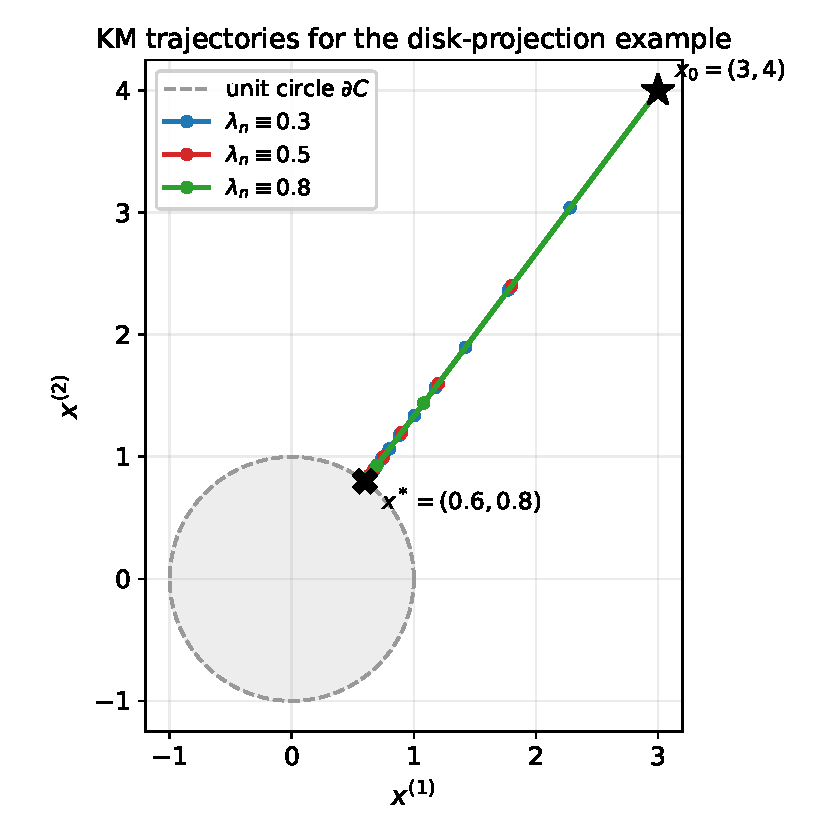
\includegraphics[width=0.78\linewidth]{km_trajectories.pdf}\\
      {\scriptsize Constant $\lambda=0.3,0.5,0.8$: converge to $x^*$
      at different speeds.}
    \end{column}
    \begin{column}{0.5\textwidth}
      \centering
      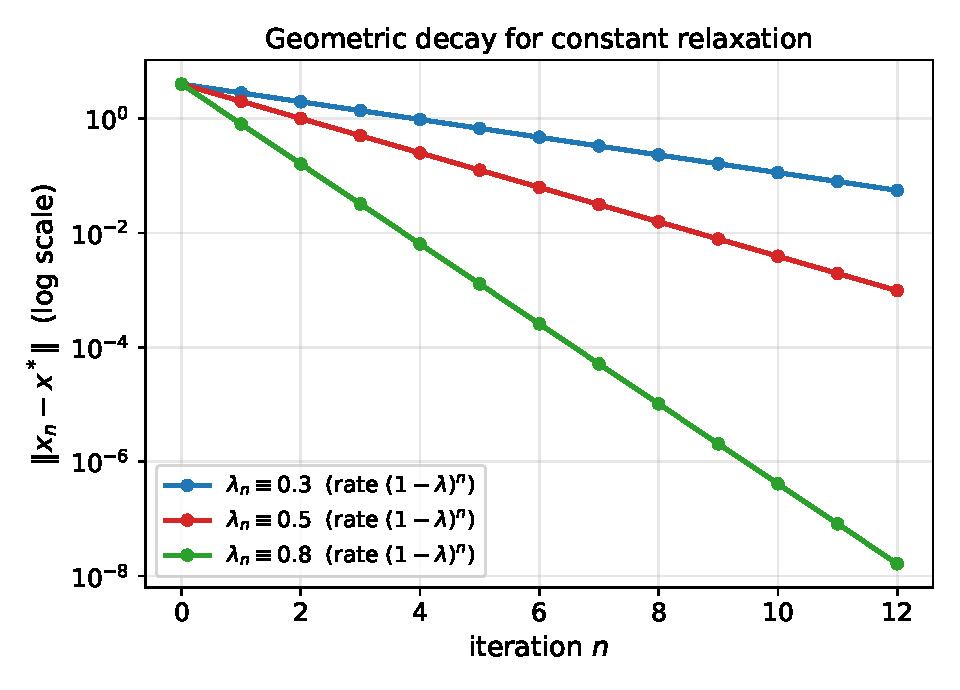
\includegraphics[width=0.78\linewidth]{km_convergence_rate.pdf}\\
      {\scriptsize $\norm{x_n-x^*}$ vs.\ $n$, log scale: straight
      lines $=$ geometric decay.}
    \end{column}
  \end{columns}
\end{frame}

\begin{frame}{Figure: Reich's Condition --- Satisfied vs.\ Violated}
  \centering
  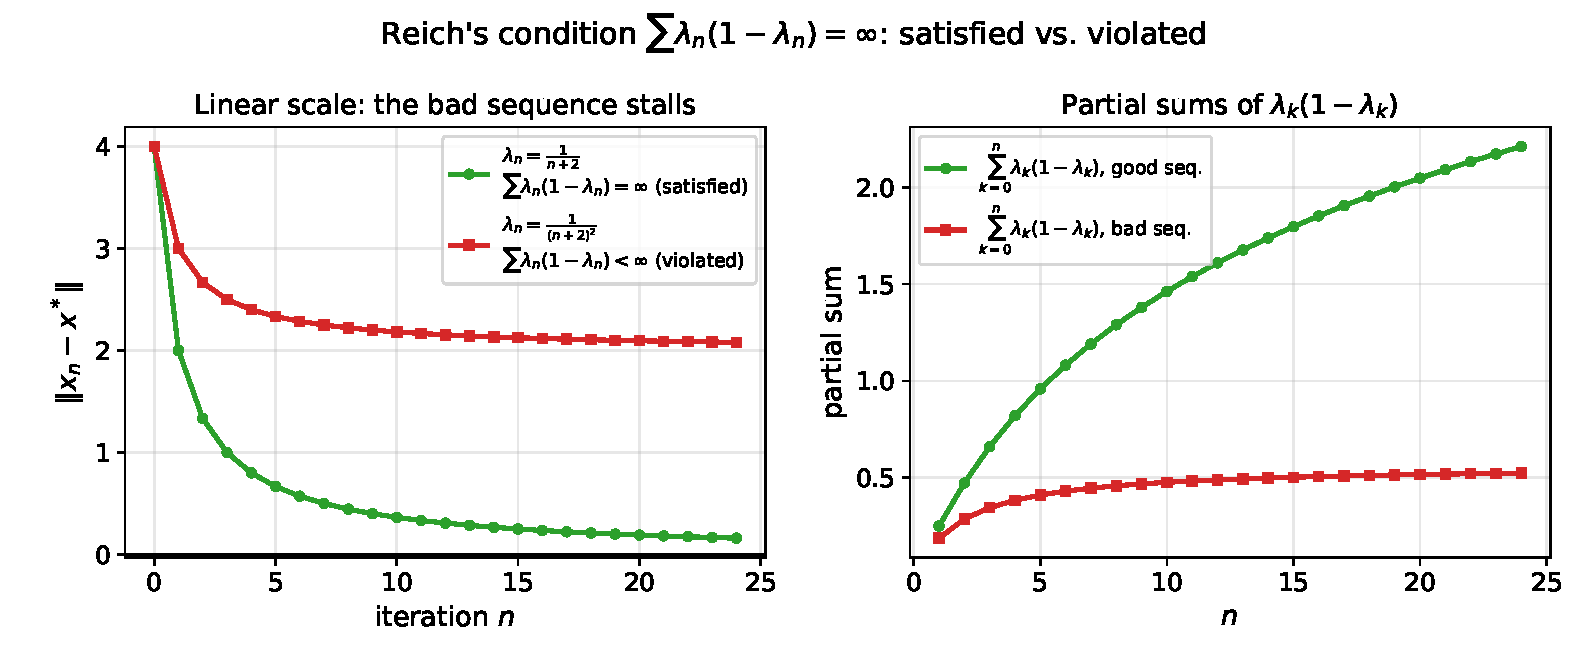
\includegraphics[width=0.92\linewidth]{km_condition_violation.pdf}\\
  {\scriptsize Left: with $\lambda_n=\frac1{n+2}$ (green) the error
  keeps shrinking toward $0$; with $\lambda_n=\frac1{(n+2)^2}$ (red) it
  stalls near $2$. Right: partial sums of $\lambda_k(1-\lambda_k)$ ---
  one keeps growing (diverges), the other flattens out (converges).}
\end{frame}

\begin{frame}[allowframebreaks]{3.2 Step-by-Step: Proof Sketch of the Fej\'er-Type Estimate}

  We derive the key inequality underlying Theorem 3.6 (and reused for
  Theorem 3.9 later) in a Hilbert space, where the computation is
  cleanest. Fix $p\in\Fix(T)$.

  \textbf{Step 1 (expand the square).} Using
  $\norm{(1-\lambda)a+\lambda b}^2=(1-\lambda)\norm{a}^2+\lambda\norm{b}^2
  -\lambda(1-\lambda)\norm{a-b}^2$ (the parallelogram-type identity, valid
  in Hilbert spaces for any $a,b\in\cH,\ \lambda\in\R$) with
  $a=x_n-p$, $b=T(x_n)-p$, $\lambda=\lambda_n$:
  $$\norm{x_{n+1}-p}^2=(1-\lambda_n)\norm{x_n-p}^2+\lambda_n\norm{T(x_n)-p}^2
    -\lambda_n(1-\lambda_n)\norm{x_n-T(x_n)}^2.$$

  \textbf{Step 2 (use nonexpansiveness).} Since $T(p)=p$,
  $\norm{T(x_n)-p}=\norm{T(x_n)-T(p)}\le\norm{x_n-p}$, so
  $$\norm{x_{n+1}-p}^2\le\norm{x_n-p}^2-\lambda_n(1-\lambda_n)\norm{x_n-T(x_n)}^2.$$
  This is the crucial \textbf{quasi-Fej\'er / Fej\'er-monotone}
  inequality: it says $\norm{x_n-p}^2$ decreases by \emph{at least}
  $\lambda_n(1-\lambda_n)\norm{x_n-T(x_n)}^2$ at every step.

  \framebreak

  \textbf{Step 3 (telescope and sum).} Summing Step 2's inequality for
  $n=0,\dots,N-1$ telescopes the left side:
  $$\sum_{n=0}^{N-1}\lambda_n(1-\lambda_n)\norm{x_n-T(x_n)}^2
    \le\norm{x_0-p}^2-\norm{x_N-p}^2 \le \norm{x_0-p}^2.$$
  Since the right-hand side is bounded uniformly in $N$, letting
  $N\to\infty$ gives
  $$\sum_{n=0}^{\infty}\lambda_n(1-\lambda_n)\norm{x_n-T(x_n)}^2<+\infty.$$

  \textbf{Step 4 (extract a vanishing subsequence).} Because
  $\sum_n\lambda_n(1-\lambda_n)=+\infty$ by hypothesis, but the weighted
  sum above with weights $\lambda_n(1-\lambda_n)$ and terms
  $\norm{x_n-T(x_n)}^2$ is finite, the terms $\norm{x_n-T(x_n)}^2$
  cannot stay bounded away from $0$: we get
  $\liminf_{n\to\infty}\norm{x_n-T(x_n)}=0$.

  \framebreak

  \textbf{Step 5 (upgrade liminf to full limit).} Combine with property
  (ii) from before: $\norm{x_n-T(x_n)}$ is a \emph{monotone
  non-increasing} sequence. A monotone sequence with a subsequence
  going to $0$ must itself converge to $0$:
  $$\lim_{n\to\infty}\norm{x_n-T(x_n)}=0.$$

  \textbf{Step 6 (weak cluster points are fixed points).} $\{x_n\}$ is
  bounded (by Step 1's monotonicity of $\norm{x_n-p}$), so it has weak
  cluster points; using demiclosedness of $\operatorname{Id}-T$ at $0$
  (a standard fact for nonexpansive $T$) and Step 5, every weak cluster
  point lies in $\Fix(T)$.

  \textbf{Step 7 (Opial argument closes the loop).} Fej\'er monotonicity
  (Step 1's consequence, property (i)) plus Opial's property forces
  \emph{all} weak cluster points to coincide $\Rightarrow$ $\{x_n\}$
  itself converges weakly to a single point of $\Fix(T)$. $\blacksquare$
\end{frame}

\begin{frame}[allowframebreaks]{3.2 Strong Convergence and Related Results}

  Weak convergence is often all one can hope for in infinite dimensions
  with nonexpansive $T$; strong (norm) convergence needs an extra
  structural assumption on $T$.

  \begin{block}{Theorem 3.7 (\emph{[195, Thm.\ 1]})}
    Let $X$ be a real uniformly convex Banach space, $C\subset X$
    closed convex, $T:C\to C$ nonexpansive with $\Fix(T)\ne\emptyset$.
    Suppose $S:=\operatorname{Id}-T$ is \textbf{$\varphi$-accretive} and
    $\{\lambda_n\}$ satisfies $\sum_{n=0}^{+\infty}\lambda_n(1-\lambda_n)=+\infty$.
    Then $\{x_n\}$ from (3.1) \textbf{converges in norm} to a fixed
    point of $T$.
  \end{block}
  ($\varphi$-accretivity of $\operatorname{Id}-T$ is a quantitative
  strengthening of monotonicity that rules out the ``flat'' directions
  responsible for merely-weak convergence.) The uniform convexity
  hypothesis can be relaxed to strict convexity + the Kadec--Klee
  property, together with demiclosedness of $S$ and $\lambda_n\le c<1$,
  $\sum\lambda_n=+\infty$.

  \begin{block}{Open Problem (Xu)}
    For a uniformly convex Banach space $X$, closed bounded convex
    $C$, nonexpansive $T:C\to C$ with $\Fix(T)\ne\emptyset$, and
    $\{\lambda_n\}\subset[0,1]$ with $\sum\lambda_n(1-\lambda_n)=+\infty$:
    does the KM sequence $\{x_n\}$ from (3.1) always converge to a
    fixed point of $T$ (in the sense of Theorem 3.6, but \emph{without}
    Fr\'echet differentiability / Opial)?
  \end{block}

  \framebreak

  \textbf{A continuous-time viewpoint (Bo\c t \& Csetnek).} Let
  $\lambda:[0,+\infty)\to[0,1]$ be Lebesgue measurable, $x_0\in\cH$.
  \begin{block}{Dynamical system (3.10)}
    $$\dot x(t)=\lambda(t)\bigl(T(x(t))-x(t)\bigr), \qquad x(0)=x_0.$$
  \end{block}
  Explicit Euler discretization with step size $h_n$:
  $x_{n+1}=x_n+h_n\lambda_n(T(x_n)-x_n)$; taking $h_n\equiv1$ recovers
  the KM iteration (3.1) exactly. So (3.1) is literally a
  \emph{time-1 Euler step} of this ODE.

  \begin{block}{Theorem 3.8}
    If $\int_0^{+\infty}\lambda(t)(1-\lambda(t))\,dt=+\infty$ \textbf{or}
    $\inf_{t\ge0}\lambda(t)>0$, then the unique strong global solution
    $x(t)$ satisfies $\lim_{t\to+\infty}(T(x(t))-x(t))=0$ and $x(t)$
    converges weakly to a point of $\Fix(T)$, with rate
    $$\norm{T(x(t))-x(t)}\le\frac{d(x_0,\Fix T)}{\sqrt{\underline\tau\, t}},
    \qquad \underline\tau:=\inf_{t\ge0}\lambda(t)(1-\lambda(t))>0,$$
    i.e.\ an $o(1/\sqrt t)$ (in fact quantitative $O(1/\sqrt t)$) rate ---
    the continuous-time ancestor of the discrete rates in Section 3.4.
  \end{block}
\end{frame}

\begin{frame}[fragile]{Python: Section 3.2 --- Verifying Reich's Condition Numerically}
  \begin{lstlisting}[style=python]
import numpy as np

def T(x):
    n = np.linalg.norm(x)
    return x / n if n > 1 else x

def km_orbit(lam_fn, x0, n_steps):
    x = np.array(x0, dtype=float)
    hist = [x.copy()]
    for n in range(n_steps):
        lam = lam_fn(n)
        x = (1 - lam) * x + lam * T(x)
        hist.append(x.copy())
    return np.array(hist)

xstar = np.array([0.6, 0.8])
good = lambda n: 1.0 / (n + 2)          # sum lam(1-lam) = +infinity
bad  = lambda n: 1.0 / (n + 2) ** 2     # sum lam(1-lam) < +infinity
for name, lam_fn in [("good", good), ("bad", bad)]:
    orbit = km_orbit(lam_fn, [3.0, 4.0], 24)
    err = np.linalg.norm(orbit - xstar, axis=1)
    psum = sum(lam_fn(n) * (1 - lam_fn(n)) for n in range(24))
    print(f"{name}: final err={err[-1]:.4f}, sum lam(1-lam)={psum:.4f}")
# good: final err -> 0 (Reich's condition holds)
# bad : final err -> ~2.08 (condition fails, iteration stalls)
  \end{lstlisting}
\end{frame}

% =================================================================
\section{3.3 KM Iteration with Perturbations}
% =================================================================

\begin{frame}[allowframebreaks]{3.3 Why Perturbations?}

  \textbf{Motivation.} In practice, $T(x_n)$ is rarely evaluated
  exactly: floating-point error, inexact subroutines, or deliberately
  injected corrections (e.g.\ for \emph{superiorization}, or building
  \emph{inertial} accelerations on top of KM) all add a small error term
  at each step. We want conditions under which convergence
  \emph{survives} such perturbations.

  \begin{block}{Perturbed KM iteration (3.11), Dong et al.}
    $$x_{n+1}=(1-\lambda_n)(x_n+e_n^1)+\lambda_n T(x_n+e_n^2)
      \quad\text{for each } n\ge0,$$
    where $e_n^1,e_n^2\in\cH$ are the perturbations injected into the
    ``keep'' branch and the ``move'' branch respectively.
  \end{block}

  \begin{block}{Summability condition (3.12)}
    $$\sum_{n=0}^{\infty}\norm{e_n^i}<+\infty \quad\text{for each } i=1,2.$$
  \end{block}
  \textbf{Plain terms:} the \emph{total} amount of error injected over
  all (infinitely many) iterations must be finite --- individual errors
  can be nonzero forever, but they must shrink fast enough that their
  sum converges (e.g.\ $\norm{e_n^i}=O(1/n^{1+\varepsilon})$ works;
  $\norm{e_n^i}=O(1/n)$ does \emph{not}, since $\sum 1/n$ diverges).

  \framebreak

  \textbf{Intuition: why summable, not just vanishing?} If merely
  $e_n^i\to0$ (but not summable, e.g.\ $\Theta(1/n)$), the errors can
  still accumulate an \emph{unbounded} total drift, exactly as a random
  walk with shrinking-but-not-summable steps can still wander off to
  infinity. Summability guarantees the cumulative nuisance is bounded,
  so the ``clean'' Fej\'er-monotonicity argument of Section 3.2 only
  picks up a bounded correction term, which does not destroy weak
  convergence.
\end{frame}

\begin{frame}[allowframebreaks]{3.3 Lemma 3.1: Residual Bound Under Perturbation}

  \begin{block}{Lemma 3.1}
    Let $T:\cH\to\cH$ be nonexpansive and $\{x_n\}$ generated by (3.11).
    Then
    $$\norm{x_{n+1}-T(x_{n+1})}\le\norm{x_n-T(x_n)}+2\bigl(\norm{e_n^1}+\norm{e_n^2}\bigr)
    \quad\text{for each } n\ge0.$$
  \end{block}

  \textbf{Step-by-step proof.}

  \textbf{Step 1.} Write out $x_{n+1}-T(x_{n+1})$ using (3.11) and
  regroup:
  \begin{align*}
    x_{n+1}-T(x_{n+1})
    &=(1-\lambda_n)\bigl[(x_n+e_n^1)-T(x_n+e_n^2)\bigr]\\
    &\quad+\bigl[T(x_n+e_n^2)-T\bigl((1-\lambda_n)(x_n+e_n^1)+\lambda_nT(x_n+e_n^2)\bigr)\bigr].
  \end{align*}

  \textbf{Step 2.} Apply the triangle inequality, then nonexpansiveness
  of $T$ to the second bracket (note the argument of the outer $T$ is
  exactly $x_{n+1}$):
  \begin{align*}
    \norm{x_{n+1}-T(x_{n+1})}
    &\le(1-\lambda_n)\norm{(x_n+e_n^1)-T(x_n+e_n^2)}\\
    &\quad+\norm{T(x_n+e_n^2)-T(x_{n+1})}\\
    &\le(1-\lambda_n)\norm{(x_n+e_n^1)-T(x_n+e_n^2)}\\
    &\quad+\lambda_n\norm{(x_n+e_n^1)-T(x_n+e_n^2)}+\norm{e_n^1}+\norm{e_n^2}\\
    &= \norm{(x_n+e_n^1)-T(x_n+e_n^2)}+\norm{e_n^1}+\norm{e_n^2}.
  \end{align*}

  \framebreak

  \textbf{Step 3.} Bound the perturbed residual by the clean one, again
  via nonexpansiveness applied twice:
  $$\norm{(x_n+e_n^1)-T(x_n+e_n^2)}
  \le\norm{x_n-T(x_n)}+\norm{e_n^1}+\norm{e_n^2}.$$

  \textbf{Step 4.} Combine Steps 2--3:
  $$\norm{x_{n+1}-T(x_{n+1})}\le\norm{x_n-T(x_n)}+2\bigl(\norm{e_n^1}+\norm{e_n^2}\bigr). \qquad\blacksquare$$

  \textbf{Reading it:} the fixed-point residual can only grow by (twice)
  the size of the perturbations injected at that step --- so under the
  summability condition (3.12), the residual's growth over all time is
  bounded, which is exactly the leverage used in Theorem 3.9's proof.
\end{frame}

\begin{frame}[allowframebreaks]{3.3 Theorem 3.9: Weak Convergence with Perturbations}

  \begin{block}{Theorem 3.9}
    Let $T:\cH\to\cH$ be nonexpansive with $\Fix(T)\ne\emptyset$.
    Assume $\sum_{n=0}^{\infty}\lambda_n(1-\lambda_n)=\infty$. Then
    $\{x_n\}$ generated by the perturbed KM iteration (3.11)
    \textbf{weakly converges} to a point in $\Fix(T)$.
  \end{block}

  \textbf{Proof sketch (mirrors Section 3.2, absorbing the perturbation).}

  \textbf{Step 1.} Expand $\norm{x_{n+1}-p}^2$ using the same Hilbert
  identity as before, then bound each nonexpansive image using the
  elementary inequality
  $\norm{y+e}\le(1+\norm e)\norm y + \norm e$ (\emph{Lemma 2.9} in the
  book), to control the effect of $e_n^1,e_n^2$:
  $$\norm{x_{n+1}-p}^2\le(1+\norm{e_n^1}+\norm{e_n^2})\norm{x_n-p}^2
  +\bigl(\norm{e_n^1}+\norm{e_n^2}+\norm{e_n^1}^2+\norm{e_n^2}^2\bigr)$$
  $$\qquad -\lambda_n(1-\lambda_n)\norm{(x_n+e_n^1)-T(x_n+e_n^2)}^2.$$

  \framebreak

  \textbf{Step 2.} Because $\sum_n(\norm{e_n^1}+\norm{e_n^2})<\infty$ by
  (3.12), a discrete Gronwall-type lemma (\emph{Lemma 2.8}) applied to
  the recursion of Step 1 shows $\lim_n\norm{x_n-p}$ \textbf{exists}
  (hence $\{x_n\}$ is bounded), \emph{despite} the multiplicative
  $(1+\norm{e_n^1}+\norm{e_n^2})$ factor --- summability keeps the
  cumulative inflation finite.

  \textbf{Step 3.} Rearranging Step 1 and summing over $n$ (as in
  Section 3.2's Step 3) gives
  $$\sum_{n=0}^\infty \lambda_n(1-\lambda_n)\norm{(x_n+e_n^1)-T(x_n+e_n^2)}^2<+\infty,$$
  so, since $\sum_n\lambda_n(1-\lambda_n)=\infty$,
  $\liminf_n\norm{(x_n+e_n^1)-T(x_n+e_n^2)}=0$.

  \textbf{Step 4.} Using nonexpansiveness once more,
  $\norm{x_n-T(x_n)}\le\norm{(x_n+e_n^1)-T(x_n+e_n^2)}+\norm{e_n^1}+\norm{e_n^2}$,
  so $\liminf_n\norm{x_n-T(x_n)}=0$ too (the $e_n^i\to0$ since summable).

  \framebreak

  \textbf{Step 5.} Combine Step 4 with Lemma 3.1 (the residual can only
  grow by a \emph{summable} amount each step) to upgrade the liminf to
  a genuine limit:
  $$\lim_{n\to\infty}\norm{x_n-T(x_n)}=0.$$

  \textbf{Step 6.} $\{x_n\}$ bounded (Step 2) $\Rightarrow$ nonempty set
  $\omega_w(x_n)$ of weak cluster points; demiclosedness of
  $\operatorname{Id}-T$ plus Step 5 give $\omega_w(x_n)\subseteq\Fix(T)$.

  \textbf{Step 7.} A (perturbed) Opial-type uniqueness-of-weak-limit
  argument forces $\omega_w(x_n)$ to be a single point $\Rightarrow$
  $\{x_n\}$ converges weakly to a point of $\Fix(T)$. $\blacksquare$

  \textbf{Takeaway:} the same relaxation condition
  $\sum\lambda_n(1-\lambda_n)=\infty$ that drives clean convergence
  \emph{also} suffices with summable perturbations --- the KM scheme is
  robust to small, well-controlled errors.
\end{frame}

\begin{frame}[allowframebreaks]{3.3 Running Example: A Concrete Perturbed Iteration}

  Take $\lambda_n\equiv0.5$ and the perturbation
  $e_n=\bigl(\tfrac{0.01}{n+1},0\bigr)$ (added once per step, i.e.\ the
  simpler inexact form $x_{n+1}=(1-\lambda_n)x_n+\lambda_n(T(x_n)+e_n)$,
  cf.\ Liang et al.'s scheme (3.25) discussed in Section 3.4).

  \begin{center}
  \begin{tabular}{c c c c}
    \toprule
    $n$ & $x_n$ (perturbed) & $\norm{x_n-x^*}$ (perturbed) & $\norm{x_n-x^*}$ (clean) \\
    \midrule
    0 & $(3.000,4.000)$ & $4.000$ & $4.000$ \\
    1 & $(1.805,2.400)$ & $2.003$ & $2.000$ \\
    2 & $(1.206,1.600)$ & $1.003$ & $1.000$ \\
    3 & $(0.905,1.199)$ & $0.503$ & $0.500$ \\
    4 & $(0.755,0.999)$ & $0.252$ & $0.250$ \\
    5 & $(0.680,0.898)$ & $0.127$ & $0.125$ \\
    6 & $(0.643,0.848)$ & $0.064$ & $0.0625$ \\
    \bottomrule
  \end{tabular}
  \end{center}

  The perturbed iterates track the clean geometric decay
  $4\cdot0.5^n$ very closely, with a small persistent offset from the
  $(0.01/(n+1),0)$ nudges in the first coordinate --- and still
  converge to $x^*=(0.6,0.8)$.

  \framebreak

  \textbf{A caveat worth stating precisely.} The sequence $0.01/(n+1)$
  used above is illustrative over a short horizon, but $\sum_n
  0.01/(n+1)$ actually \textbf{diverges} (harmonic series) --- it is
  \emph{not} summable, so it does not strictly satisfy hypothesis (3.12)
  of Theorem 3.9! Over the 6 steps shown, the geometric contraction from
  $\lambda=0.5$ dominates the slowly-growing error and convergence looks
  fine numerically. To have a perturbation that \emph{rigorously}
  satisfies (3.12) (guaranteeing convergence for \emph{all} $n$, not
  just the first few), replace it with, e.g., a genuinely summable
  choice such as $e_n=\bigl(\tfrac{0.01}{(n+1)^2},0\bigr)$, since
  $\sum_n 1/(n+1)^2=\pi^2/6<\infty$. This distinction --- summable
  versus merely vanishing --- is exactly the content of condition
  (3.12) and is easy to overlook in practice.
\end{frame}

\begin{frame}{Figure: Perturbed vs.\ Clean Iteration}
  \centering
  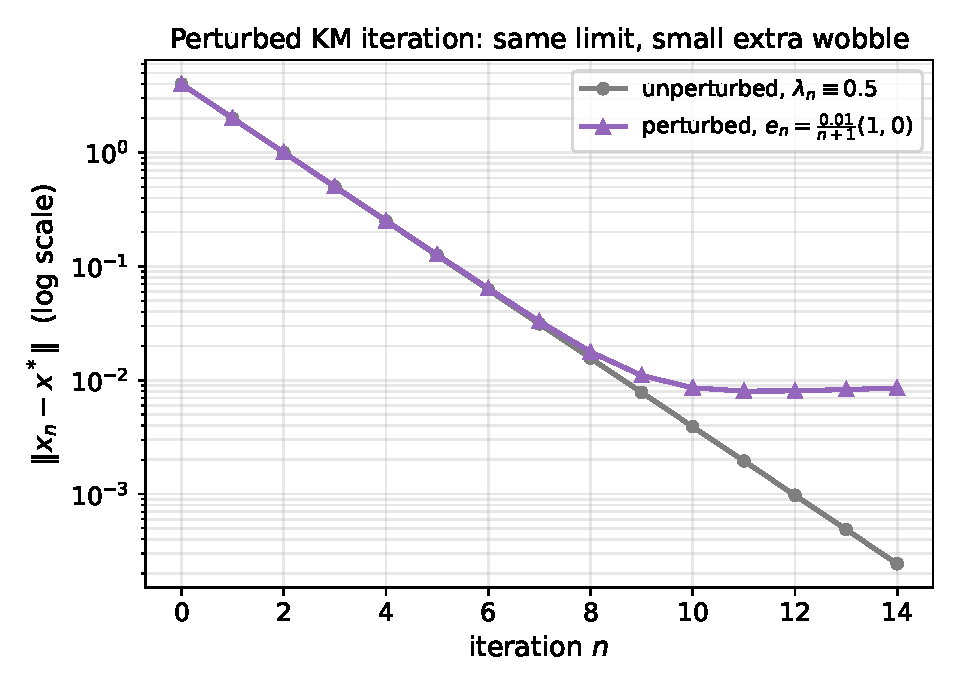
\includegraphics[width=0.62\linewidth]{km_perturbed.pdf}\\
  {\scriptsize Perturbed KM iteration ($\lambda\equiv0.5$,
  $e_n=\frac{0.01}{n+1}(1,0)$) tracks the clean geometric decay closely
  and reaches the same fixed point $x^*=(0.6,0.8)$.}
\end{frame}

\begin{frame}[allowframebreaks]{3.3 Bounded Perturbation Resilience (BPR) and Superiorization}

  \textbf{Motivation.} If an algorithm is known to be robust to
  \emph{any} sufficiently small, summable perturbation, one can
  deliberately inject perturbations that steer the iterates toward a
  \emph{secondary} objective (e.g.\ regularization) without destroying
  convergence to the original solution set --- this is the
  \emph{superiorization} methodology.

  \begin{block}{Definition 3.2 (Bounded Perturbation Resilience, BPR)}
    Let $\Theta\subseteq\cH$ and let $\mathbf A_\Psi:\Theta\to\cH$ be an
    algorithmic operator such that the \textbf{basic algorithm} (3.20)
    $$x_{n+1}=\mathbf A_\Psi(x_n), \qquad x_0\in\Theta,$$
    converges to a point in a solution set $\Psi$. $\mathbf A_\Psi$ is
    \textbf{bounded perturbations resilient} if, for \emph{any}
    $y_0\in\Theta$, the perturbed sequence
    $$y_{n+1}=\mathbf A_\Psi(y_n+\rho_n v_n), \qquad n\ge0,$$
    also converges to a point of $\Psi$, provided:
    \begin{enumerate}
      \item[(a)] $\{v_n\}$ is bounded;
      \item[(b)] $\{\rho_n\}\subset\R$ is positive with $\sum_n\rho_n<\infty$;
      \item[(c)] $y_n+\rho_n v_n\in\Theta$ for each $n\ge0$ (only needed
        when $\Theta\ne\cH$).
    \end{enumerate}
  \end{block}

  \framebreak

  \textbf{Applying this to KM.} Take $\mathbf A_\Psi^n=(1-\lambda_n)\operatorname{Id}+\lambda_n T$
  (the right-hand side of (3.1) itself). Its bounded perturbation
  (3.22) is
  $$x_{n+1}=\mathbf A^n_\Psi(x_n+\rho_n v_n)=(1-\lambda_n)(x_n+\rho_nv_n)+\lambda_nT(x_n+\rho_nv_n).$$
  Setting $e_n^1=e_n^2=\rho_nv_n$ turns this into exactly the perturbed
  scheme (3.11), and $\sum_n\rho_n<\infty$ plus boundedness of $\{v_n\}$
  gives $\sum_n\norm{e_n^i}<\infty$: condition (3.12) holds automatically!

  \begin{block}{Theorem 3.10}
    Let $T:\cH\to\cH$ be nonexpansive with $\Fix(T)\ne\emptyset$ and
    $\sum_{n=0}^{\infty}\lambda_n(1-\lambda_n)=\infty$. Then $\{x_n\}$
    from the bounded-perturbation scheme (3.22) weakly converges to a
    point of $\Fix(T)$.
  \end{block}

  \textbf{Remark 3.1.} (1) The KM iteration for nonexpansive operators
  is therefore bounded perturbations resilient --- a direct corollary of
  Theorem 3.9. (2) This BPR property is precisely the ``certificate''
  needed to justify superiorized/inertial variants of KM built on top
  of the basic scheme.
\end{frame}

\begin{frame}[fragile]{Python: Section 3.3 --- Perturbed KM and Summability}
  \begin{lstlisting}[style=python]
import numpy as np

def T(x):
    n = np.linalg.norm(x)
    return x / n if n > 1 else x

def perturbed_km(x0, n_steps, lam=0.5, err_power=1.0, err_scale=0.01):
    """x_{n+1} = (1-lam) x_n + lam (T(x_n) + e_n),
       e_n = err_scale / (n+1)**err_power * (1, 0)."""
    x = np.array(x0, dtype=float)
    hist = [x.copy()]
    for n in range(n_steps):
        e_n = np.array([err_scale / (n + 1) ** err_power, 0.0])
        x = (1 - lam) * x + lam * (T(x) + e_n)
        hist.append(x.copy())
    return np.array(hist)

xstar = np.array([0.6, 0.8])
# NOT summable: err_power=1.0 (sum 1/(n+1) diverges) -- (3.12) violated
orbit_bad = perturbed_km([3.0, 4.0], 6, err_power=1.0)
# summable: err_power=2.0 (sum 1/(n+1)^2 = pi^2/6 < infinity) -- (3.12) holds
orbit_good = perturbed_km([3.0, 4.0], 6, err_power=2.0)
for n in range(7):
    print(n, np.linalg.norm(orbit_bad[n]-xstar),
             np.linalg.norm(orbit_good[n]-xstar))
  \end{lstlisting}
\end{frame}

% =================================================================
\section{3.4 The Convergence Rate}
% =================================================================

\begin{frame}[allowframebreaks]{3.4 Why Rates Matter, and the Lipschitz Case}

  \textbf{Motivation.} Weak/strong convergence tells us $\{x_n\}$
  \emph{eventually} reaches $\Fix(T)$, but says nothing about \emph{how
  many} iterations are needed for a target accuracy. Convergence rate
  results quantify this.

  \begin{block}{Theorem 3.11 (He et al.)}
    Let $T:\cH\to\cH$ be $L$-Lipschitz with $-T$ monotone, and
    $\lambda_n\equiv\lambda$ with
    $\max\Bigl\{\dfrac{L^2-1}{L^2+1},0\Bigr\}<\lambda<1$. Then, with
    $x^*$ the unique fixed point,
    $$\norm{x_n-x^*}\le\frac{[\lambda^2+(1-\lambda)^2L^2]^{n/2}}
      {1-\sqrt{\lambda^2+(1-\lambda)^2L^2}}\,\norm{x_1-x_0}.$$
    Choosing the \emph{optimal} $\lambda=\dfrac{L^2}{L^2+1}$ gives the
    (essentially) optimal geometric rate
    $$\norm{x_n-x^*}\le\sqrt{L^2+1}\,\bigl(1+\sqrt{L^2+1}\bigr)
      \left(\frac{L}{\sqrt{L^2+1}}\right)^{n}\norm{x_1-x_0}.$$
  \end{block}
  \textbf{Reading it:} under this extra Lipschitz/monotonicity
  structure, KM converges \emph{geometrically} (linearly) --- our
  constant-$\lambda$ running example already showed this behaviour, but
  Theorem 3.11 makes the base of the geometric rate explicit in terms
  of $L$ and the optimal choice of $\lambda$.

  \framebreak

  \textbf{The harder, general case.} For a merely nonexpansive $T$
  (no Lipschitz constant beyond 1, no extra monotonicity), there is in
  general \textbf{no} rate on $\norm{x_n-x^*}$ itself. The workhorse
  quantity instead is the \textbf{fixed-point residual}
  $\norm{x_n-T(x_n)}$, whose convergence to $0$ is called
  \textbf{asymptotic regularity} (recall this quantity is exactly the
  one shown monotone non-increasing in property (ii), Section 3.2).

  Goebel and Kirk showed: for every $\varepsilon>0$,
  $\norm{x_n-T(x_n)}\le\varepsilon$ for all $n\ge n_0(\varepsilon,C)$,
  with $n_0$ independent of $x_0$ and $T$ (later refined so $n_0$
  depends on $C$ only through its diameter).
\end{frame}

\begin{frame}[allowframebreaks]{3.4 The Sharp $O(1/\sqrt n)$ Rate}

  Baillon and Bruck first showed, for constant $\lambda_n\equiv\lambda$
  on a bounded $C$, the rate $\norm{x_n-T(x_n)}=O(1/\log n)$, later
  conjecturing a universal constant $\kappa$ with
  \begin{equation*}
  \norm{x_n-T(x_n)}\le\kappa\,\frac{\operatorname{diam}(C)}{\sqrt{\sum_{i=0}^n\lambda_i(1-\lambda_i)}}. \tag{3.23}
  \end{equation*}

  \textbf{Reading (3.23) in plain terms:} the fixed-point residual is
  controlled by $1/\sqrt{\cdot}$ of the \emph{same} quantity
  $\sum\lambda_i(1-\lambda_i)$ from Reich's condition. This is precisely
  what ``$O(1/\sqrt n)$'' means here: if $\sum_{i=0}^n\lambda_i(1-\lambda_i)$
  grows proportionally to $n$ (e.g.\ constant $\lambda$, so each term
  contributes a fixed positive amount), the residual shrinks like a
  constant divided by $\sqrt n$ --- doubling $n$ shrinks the guaranteed
  bound by only $1/\sqrt2$.

  For affine $T$ and $\lambda_n\equiv1/2$: tight bound with
  $\kappa=1/\sqrt{2\pi}$; for general $\lambda_n$, optimal constant
  $\kappa=\max_{x\ge0}\sqrt x\,e^{-x}I_0(x)\sim0.4688$ ($I_0$: modified
  Bessel function of the first kind).

  \framebreak

  \begin{block}{Theorem 3.12 (Bravo \& Cominetti, \emph{[26, Thm.\ 1.1]})}
    The constant $\kappa=1/\sqrt\pi$ in (3.23) is \textbf{tight}: for
    every $\kappa<1/\sqrt\pi$ there exist a nonexpansive $T$ on the unit
    cube $C=[0,1]^{\N}\subseteq\ell^\infty(\N)$, an initial point
    $x_0\in C$, and a constant $\lambda_n\equiv\lambda$, such that for
    some $n\ge0$,
    $$\norm{x_n-T(x_n)}>\kappa\,\frac{\operatorname{diam}(C)}{\sqrt{\sum_{i=0}^n\lambda_i(1-\lambda_i)}}.$$
  \end{block}
  So (3.23) with $\kappa=1/\sqrt\pi$ is the best possible constant that
  can hold for \emph{all} nonexpansive maps and constant relaxations ---
  no universal improvement is possible.

  \begin{block}{Theorem 3.13 (Matsushita, \emph{[148, Thm.\ 3.1]})}
    Let $C\subset\cH$ be closed, $T:C\to C$ nonexpansive with
    $\Fix(T)\ne\emptyset$, $\{x_n\}$ from (3.1) with $\{\lambda_n\}
    \subset[0,1]$. If $\sigma_n:=\sum_{j=0}^n\lambda_j(1-\lambda_j)\to\infty$,
    then $$\norm{x_n-T(x_n)}=o(1/\sqrt{\sigma_n}),\quad\text{i.e.}\quad
    \lim_{n\to\infty}\sqrt{\sigma_n}\,\norm{x_n-T(x_n)}=0.$$
  \end{block}
  This upgrades the big-$O$ bound (3.23) to \textbf{little-o}: not only
  bounded by a constant times $1/\sqrt{\sigma_n}$, but the product
  actually vanishes in the limit.
\end{frame}

\begin{frame}[allowframebreaks]{3.4 Complexity Bounds for the Perturbed Iteration}

  Liang et al.\ studied the inexact iteration
  \begin{equation*}
  x_{n+1}=(1-\lambda_n)x_n+\lambda_n\bigl(T(x_n)+e_n\bigr), \quad n\ge1. \tag{3.25}
  \end{equation*}
  and Dong et al.\ extended their pointwise/ergodic bounds to the fully
  perturbed scheme (3.11) (which contains (3.25) as the special case
  $e_n^1=0$, $e_n^2=e_n$).

  \textbf{Setup.} Let
  $\overline\tau=\sup_n\lambda_n(1-\lambda_n)$,
  $\underline\tau=\inf_n\lambda_n(1-\lambda_n)$,
  $d_1=d(x_1,\Fix(T))$, and define bounded auxiliary constants
  $\upsilon_1,\upsilon_2,\upsilon_3$ collecting suprema of residuals and
  perturbation norms (full definitions in (3.11)-preceding text).

  \begin{block}{Theorem 3.14 (Pointwise Iteration-Complexity Bound)}
    If $0<\inf_n\lambda_n\le\sup_n\lambda_n<1$ and
    $\{(n+1)(\norm{e_n^1}+\norm{e_n^2})\}\in\ell^1_+$ (i.e.\ that
    weighted series converges), then, with $C_1$ a finite constant built
    from $\upsilon_1,\upsilon_2,\upsilon_3$ and the perturbation series,
    $$\norm{x_n-T(x_n)}\le\sqrt{\frac{d_1^2+C_1}{\underline\tau\,(n+1)}}.$$
  \end{block}
  This is precisely an $O(1/\sqrt n)$ pointwise rate for the residual,
  \emph{including} the effect of summable perturbations (through $C_1$).

  \framebreak

  \begin{block}{Theorem 3.15 (Ergodic Iteration-Complexity Bound)}
    With $\Lambda_n=\sum_{j=0}^n\lambda_j$ and
    $C_2=\sum_{n=0}^\infty\bigl[(1-\lambda_n)\norm{e_n^1}+\lambda_n\norm{e_n^2}\bigr]<\infty$,
    $$\Bigl\|\frac{1}{\Lambda_n}\sum_{j=0}^n\lambda_j\bigl(x_j-T(x_j)\bigr)\Bigr\|
      \le\frac{2(d_1+C_2)}{\Lambda_n}.$$
    In particular, if $\inf_n\lambda_n>0$, then
    $\Lambda_n=\Theta(n)$ and the ergodic (weighted-average) residual is
    $O(1/n)$ --- \emph{faster} than the $O(1/\sqrt n)$ pointwise rate,
    since averaging cancels oscillations.
  \end{block}

  \framebreak

  \textbf{Extending to inexact $T(x_n)$ in Banach spaces.} Bravo et al.
  established, for $\tau_n=\sum_{k=0}^n\lambda_k(1-\lambda_k)$ and
  $\sigma(y)=\min\{1,1/\sqrt{\pi y}\}$:

  \begin{block}{Theorem 3.16 (\emph{[27, Thm.\ 3]}) --- setup}
    $X$ Banach, $C$ closed convex, $T:C\to C$ nonexpansive, $\{x_n\}$
    from the inexact scheme (3.25) with the boundedness condition
    $x_n\in C$, $\norm{T(x_n)-x_0}\le\kappa$ for all $n$.
  \end{block}
  If additionally $\sum_n\norm{e_n}<\infty$ and $\lambda_n$ is bounded
  away from $0$ and $1$, there is a constant $c\ge0$ with
  $$\norm{x_n-T(x_n)}\le\frac{c}{\sqrt n}+\sum_{i\ge\lfloor n/2\rfloor}2\norm{e_i}.$$
  More generally, for nondecreasing $\varphi$ with
  $\mu=\sum_n\varphi(n)\norm{e_n}<\infty$:
  $$\norm{x_n-T(x_n)}\le\frac{c}{\sqrt n}+\frac{2\mu}{\varphi(\lfloor n/2\rfloor)}.$$

  \framebreak

  \textbf{Rate depends on the error's decay rate.} If
  $\norm{e_n}=O(1/n^a)$ for $a\ge\tfrac12$ and $\lambda_n$ bounded away
  from $0,1$:
  \begin{itemize}
    \item if $\tfrac12\le a<1$: $\norm{x_n-T(x_n)}=O(1/n^{a-1/2})$;
    \item if $a=1$: $\norm{x_n-T(x_n)}=O(\log n/\sqrt n)$;
    \item if $a>1$: $\norm{x_n-T(x_n)}=O(1/\sqrt n)$ (error decay no
      longer the bottleneck; recovers the unperturbed rate).
  \end{itemize}

  \textbf{A sobering closing remark.} All rates obtained so far for
  nonexpansive $T$ are only \textbf{sublinear}: fast early progress,
  then a slow tail. Oblomskaja constructed a (linear) example where
  convergence is slower than $n^{-\tau}$ for \emph{every} $\tau\in(0,1)$
  --- KM convergence for nonexpansive maps can be arbitrarily slow in
  the worst case. Relaxation strategies and inertial acceleration
  (Chapters 5--7) are the main remedies developed for this.
\end{frame}

\begin{frame}[fragile]{Python: Section 3.4 --- Empirical $O(1/\sqrt n)$ Rate}
  \begin{lstlisting}[style=python]
import numpy as np

def T(x):
    n = np.linalg.norm(x)
    return x / n if n > 1 else x

def residual_orbit(lam_fn, x0, n_steps):
    """Track the fixed-point residual ||x_n - T(x_n)|| along the KM orbit."""
    x = np.array(x0, dtype=float)
    residuals = []
    sigma = 0.0          # running sum_{k<=n} lambda_k(1-lambda_k)
    sigmas = []
    for n in range(n_steps):
        lam = lam_fn(n)
        residuals.append(np.linalg.norm(x - T(x)))
        sigma += lam * (1 - lam)
        sigmas.append(sigma)
        x = (1 - lam) * x + lam * T(x)
    return np.array(residuals), np.array(sigmas)

res, sig = residual_orbit(lambda n: 0.5, [3.0, 4.0], 40)
bound = 1.0 / np.sqrt(np.pi) * 2.0 / np.sqrt(np.maximum(sig, 1e-12))  # (3.23)-style
for n in [0, 5, 10, 20, 39]:
    print(f"n={n:3d}  residual={res[n]:.6f}  1/sqrt(pi*sigma_n) bound={bound[n]:.6f}")
# Confirms: residual stays comfortably below the O(1/sqrt(sigma_n)) envelope.
  \end{lstlisting}
\end{frame}

% =================================================================
\section{Summary}
% =================================================================

\begin{frame}[allowframebreaks]{Chapter 3 Summary}

  \begin{itemize}
    \item \textbf{3.1} The KM iteration
      $x_{n+1}=(1-\lambda_n)x_n+\lambda_nT(x_n)$ generalizes Picard
      iteration via relaxation; Mann's matrix formulation (3.2) and its
      Ces\`aro special case recover it as a diagonal-relaxation scheme
      (Dotson's normal Mann processes); Combettes--Pennanen/Glaudin push
      this to general (even sign-indefinite) concentrating arrays.
    \item \textbf{3.2} The basic Fej\'er-monotonicity properties (i)-(ii)
      are easy but insufficient; Reich's Theorem 3.6
      ($\sum\lambda_n(1-\lambda_n)=\infty$) gives weak convergence for
      nonexpansive $T$ in Hilbert/Opial spaces; strong convergence
      (Theorem 3.7) needs $\varphi$-accretivity of $\operatorname{Id}-T$.
    \item \textbf{3.3} Perturbed KM (3.11) with summable errors
      ($\sum\norm{e_n^i}<\infty$) preserves weak convergence
      (Theorem 3.9) under the \emph{same} condition on $\{\lambda_n\}$;
      this underlies bounded perturbation resilience (Definition 3.2)
      and superiorization.
    \item \textbf{3.4} Rates are sublinear in general: the sharp
      universal bound $\norm{x_n-T(x_n)}\le\frac{1}{\sqrt\pi}
      \frac{\operatorname{diam}(C)}{\sqrt{\sum_{i\le n}\lambda_i(1-\lambda_i)}}$
      (Bravo--Cominetti) is tight; perturbed/inexact versions cost an
      extra term controlled by the decay rate of $\{e_n\}$; worst-case
      convergence can be slower than any polynomial rate.
  \end{itemize}

  \textbf{Running example, one-line recap.} On the unit-disk projection
  with $x_0=(3,4)$: constant $\lambda$ gives geometric decay $4(1-\lambda)^n$;
  $\lambda_n=\tfrac1{n+2}$ gives sublinear $4/(n+1)$ decay (condition
  satisfied); $\lambda_n=\tfrac1{(n+2)^2}$ \emph{stalls} near
  $\norm{x_n-x^*}\approx2$ (condition violated); a small summable
  perturbation barely disturbs convergence to $x^*=(0.6,0.8)$.
\end{frame}

\end{document}
